\section{Extrinsic Parameters} \label{sec:extrinsics}

Next, we would like to find the extrinsic matrix, $M_{ext}$, which relates the positional vector $\vec{p}_w$ of point $P$ in the world coordinate frame, to its positional vector $\vec{p}_c$ in the camera coordinate frame. Similar to what we did in section \ref{sec:intrinsics}, we can express this in homogenous coordinates as follows:
\begin{equation}
    \widetilde{p}_c =  M_{ext}\:\widetilde{p}_w
\end{equation}

\begin{figure}[H]
    \centering
    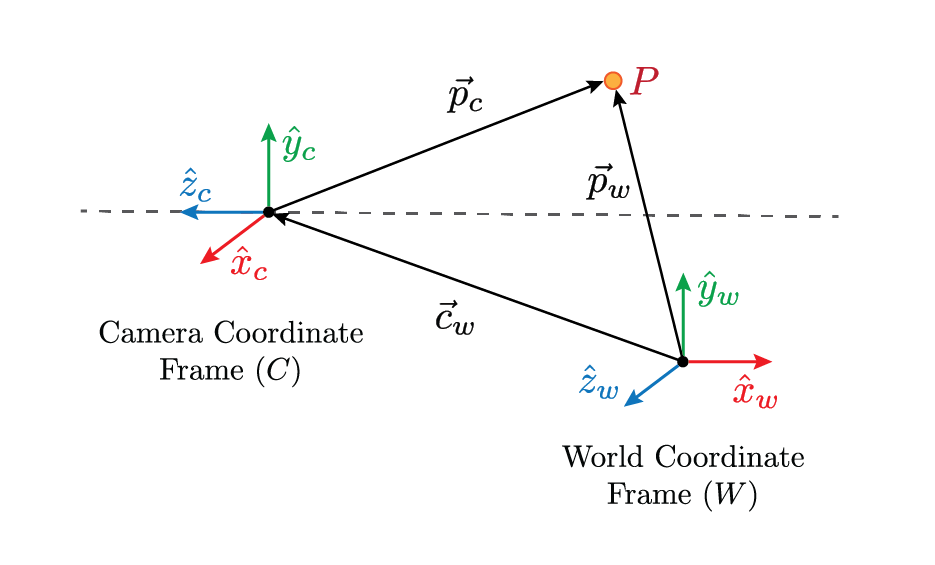
\includegraphics[width=0.9\textwidth]{figures/coord_transform}
    \caption{Coordinate transformation from the world coordinate frame to the camera frame.}
\end{figure}

For the extrinsic parameters of the camera, we have the position $\vec{c}_w$ of the camera in world coordinates and orientation $R$ of the camera. The orientation, $R$, is a 3x3 rotational matrix: 

\begin{equation}
    R = 
    \begin{bmatrix}
        r_{11} & r_{12} & r_{13} \\
        r_{21} & r_{22} & r_{23} \\
        r_{31} & r_{32} & r_{33}
    \end{bmatrix}
\end{equation}

\noindent where:
\begin{itemize}
    \item Row 1: Direction of $\hat{x}_c$ in world coordinate frame.
    \item Row 2: Direction of $\hat{y}_c$ in world coordinate frame.
    \item Row 3: Direction of $\hat{z}_c$ in world coordinate frame.
\end{itemize}

\noindent 

\begin{subequations}
    \begin{align}
        \vec{p}_c & = R(\vec{p}_w-\vec{c}_w) \\
                  & = R\vec{p}_w -R\vec{c}_w  
    \end{align}
\end{subequations}



\begin{gather}
    \vec{p}_c = R\vec{p}_w + \vec{t} \\
    \begin{bmatrix}
        x_c \\ y_c \\ z_c
    \end{bmatrix}
    =
    \begin{bmatrix}
        r_{11} & r_{12} & r_{13} \\
        r_{21} & r_{22} & r_{23} \\
        r_{31} & r_{32} & r_{33}
    \end{bmatrix}
    \begin{bmatrix}
        x_w \\ y_w \\ z_w
    \end{bmatrix}
    +
    \begin{bmatrix}
        t_x \\ t_y \\ t_z
    \end{bmatrix}
\end{gather}


\begin{equation}
    \begin{bmatrix}
        x_c \\ y_c \\ z_c \\ 1
    \end{bmatrix}
    =
    \underbrace{
        \begin{bmatrix}
            r_{11} & r_{12} & r_{13} & t_x \\
            r_{21} & r_{22} & r_{23} & t_y \\
            r_{31} & r_{32} & r_{33} & t_z \\
            0      & 0      & 0      & 1
        \end{bmatrix}
    }_{\mathlarger{=M_{ext}}}
    \begin{bmatrix}
        x_w \\ y_w \\ z_w \\1
    \end{bmatrix}
\end{equation}
